\documentclass[12pt]{report}

\usepackage[a4paper]{geometry}
%\geometry{left=2.5cm,right=2.5cm,top=2.5cm,bottom=2.5cm, a4paper}
\usepackage[utf8]{inputenc}
\usepackage{amsmath}
\usepackage{amsthm}
\usepackage{amssymb}
\usepackage{ulem}
\usepackage{graphicx}
\usepackage{caption}
\graphicspath{}
\usepackage[document]{ragged2e}
\usepackage{setspace}
\usepackage{tabularx}
\usepackage[slovene]{babel}
\usepackage{textcomp, gensymb}
\usepackage{siunitx}
\usepackage{pdfrender,xcolor}
\usepackage{hyperref}
\usepackage{xurl}
\usepackage{float}
\usepackage{titlesec}

\newfloat{slika}{htbp}{loc}
\floatname{slika}{Slika}

\newfloat{tabela}{htbp}{loc}
\floatname{tabela}{Tabela}

% Differential
\newcommand{\diff}{\mathrm{d}}

\title{
  
\includegraphics[width=0.4\textwidth]{fmf_logo}\\
  {\small Oddelek za fiziko} \\
  {Uklon svetlobe}\\
  {\small Poročilo pri fizikalnem praktikumu IV}\\

}
\date{}
\author{Kristofer Čepon Povšič\\[5 cm]
 \small  Asistenta: Jelena Vesić  \\
}


\titleformat{\chapter}[hang]{\Huge\bfseries}{\thechapter{. }}{0pt}{\Huge\bfseries}

\setlength\parindent{0pt}

\begin{document}

\setcounter{page}{2}

\maketitle

\chapter*{Uvod}

Uklon je pojav, kjer se svetloba ne giblje več premo, ampak se širi v geometrijsko senco. To se zgodi, ko imamo tipične dimenzije primerljive z valovnimi dolžinami svetlobe. Za začetek si lahko pomagamo s \emph{Huygensovim principom}, ki pravi, da lahko vsako točko, do katere je svetloba že prišla, obravnavamo kot nov točkast izvor. Ta princip ima pomanjkljivost, saj se v točkastem izvoru valovanje širi tudi nazaj. Le to sta popravila Fresnel in Kirchhoff. 

Po poenostavitvi Fresnel-Kirchhoffov enačbe in izračunom jakosti svetlobe daleč od uklonskih rež (Fraunhoferjev približek) lahko izračunamo, da je jakost svetlobe v sredini uklonskega vzorca, ki je od radija reže $r$ odvisna: 

\begin{equation}
  j(r) = j_0 \sin \left(\frac{kr^2}{4R}\right)
\end{equation}

pri čemer smo $R$ definirali kot $R^{-1} = z_f^{-1} + z_z^{-1}$. Pri tem je $z_z$ razdalja od uklonskih rež do zaslona, $z_f$ pa razdalja od rež do gorišča leče, s katero iz laserja ustvarimo približni točkovni izvor. 

Periodični ekstremi sredinske jakosti, v katerih velja 

\begin{equation}
  n = \frac{r^2}{\lambda R}
\end{equation}

pri čemer je $n$ liho število za maksimume jakosti ter sod za minimume. 

\chapter*{Naloga}

\begin{itemize}
  \item Izmeri uklonsko sliko svetlobe za zasloni z režami. Uporabi zaslone z 1, 2, 3, 5 in 10 režami. Določi relativne intenzitete uklonskih slik. Določi širino rež $D$ in razdalje med njimi $d$. 
  \item Opazuj uklon na okrogli odprtini. Določi premer odprtine $2R$.
\end{itemize} 


\begingroup
\let\clearpage\relax

\chapter*{Potrebščine}
\begin{itemize}
\item \verb+HeNe+ laser z valovno dolžino $633 \si{nm}$, nosilna plošča za laser in translator za zaslone, 
\item par prizem v nosilcu za razširitev žarka, 
\item zasloni z odprtinami, leča z nosilcem, ravno ogledalo z nosilcem, 
\item $x$ translator z montiranim fotodetektorjem in pretvornik signalov, 
\item prenosnik s programom \verb+UklSve+
\end{itemize}

\chapter*{Navodilo}

Prižgemo in pripravimo laser skupaj z različnimi zasloni, ki imajo različne laserje. Prižgemo računalnik, inicializiramo program in z vrtenjem vijaka pomikamo mizico s fotodiodo iz ene v drugo skrajno lego. Shranimo podatke za vse reže. 

Za drugi del odstrani uklonski zaslon z režo in vstavi uklonski zaslon z okroglo odprtino. Takoj za laser postavi v snop lečo in nastavi njen položaj tako, da je divergentni laserski snop še vedno centriran na zaslonki. Svetlobo usmeri v steno za laserjem. Na zaslonu dobiš uklonsko sliko, to so koncentrični temni in svetli kolobarji. Zanima nas predvsem sredina vzroca. Premikaj položaja okrogle zaslonke povzroči izmenične svetla in temna polja. 

\endgroup


\chapter*{Obdelava podatkov}

Razdalja do senzorja je 

\[
L = (200 \pm 2)\si{cm}  
\]

Narišem graf odvisnosti jakosti svetlobe od položaja senzorja za uklonske zaslone z režami 1, 2, 3 in 5. 

\begin{slika}[H]
  \centering
  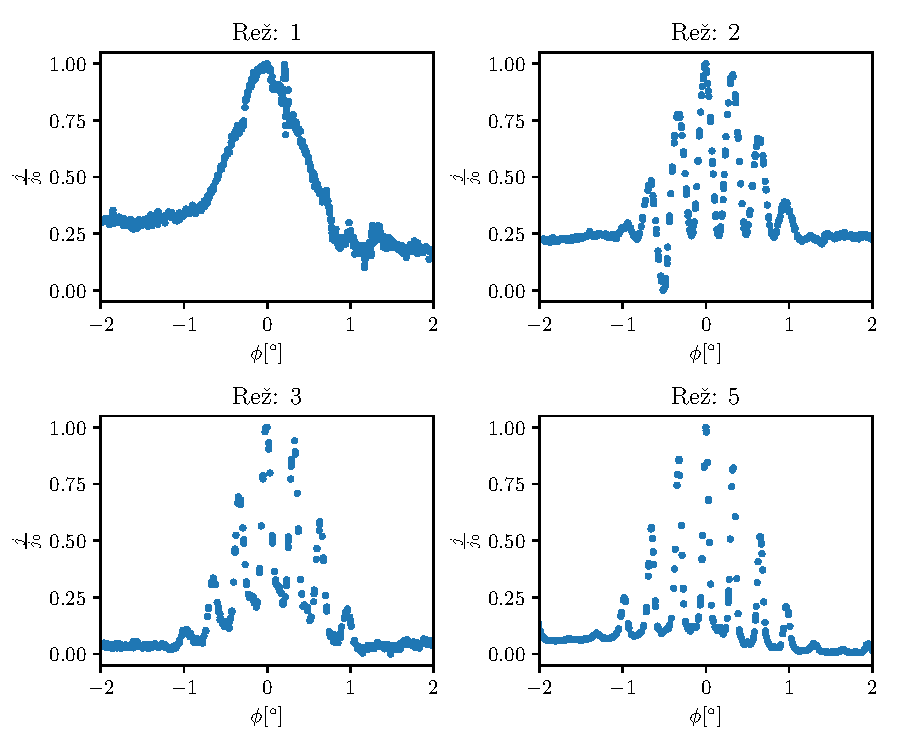
\includegraphics{reze}
  \caption{\small Izmerjene jakosti Fraunhoferjevega uklona na $n$ režah}
\end{slika}

Izračunam, da je debeline rež sledeča

\[
D = (22.0 \pm 0.1) \si{\mu m}
\]

Razdalje med režami pa so 
\begin{align*}
  d_2 &= (99.7 \pm 0.1) \si{\mu m} \\
  d_3 &= (100.1 \pm 0.3) \si{\mu m}\\
  d_5 &= (99.7 \pm 0.5) \si{\mu m}
\end{align*}

Za drugi del naloge imamo sledeče podatke: 
\begin{itemize}
  \item razdalja med lečo in režo $d_0 = (11.2 \pm 0.2) \si{cm}$
  \item razdalja med lečo in zaslonom $z_{z0} = (144.5 \pm 2) \si{cm}$
\end{itemize}

S spreminjanjem razdaljem dobim sledečo izmenjavo svetlih in temnih con: 

\begin{slika}[H]
  \centering
  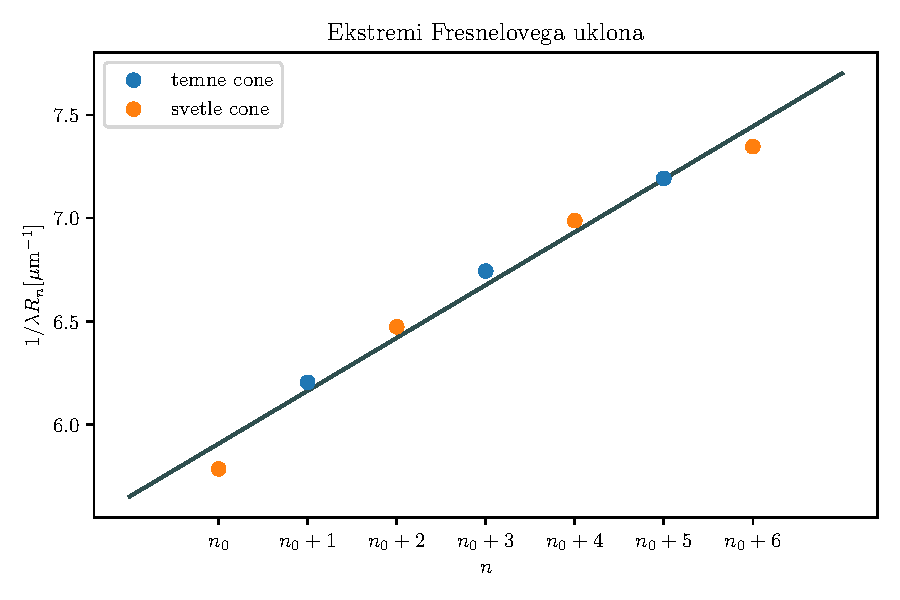
\includegraphics{fresnel-zones}
  \caption{\small Graf prikazuje vrednosti $\frac{1}{\lambda R_n}$. Svetle cone so minimumi, temne pa maksimumi jakosti. Naklon prilagojene premice je $\frac{1}{r^2}$}
\end{slika}

Radij uklonske reže je tako 
\[
r = (1.98 \pm 0.06)\si{mm}  
\]


\end{document}